\begin{center}
  \section{\capitalisewords{Next-Generation Networking and Communication Protocols for IoT}}
  Dr. Prasun Chowdhury, Associate Professor, ECE
\end{center}

\setcounter{figure}{0}
\setcounter{table}{0}

\begingroup
  \setlength{\parskip}{1pt}
  \setlength{\multicolsep}{3pt}
  \setlength{\abovecaptionskip}{1.5pt}
  \setlength{\belowcaptionskip}{1.5pt}

\begin{multicols}{2}

  \begin{abstract}
    \bfseries
    The Internet of Things (IoT) connects sensors, actuators, embedded processors, gateways, cloud platforms, and intelligent applications into large-scale cyber-physical systems. Its success depends on networking technologies that can accommodate constrained hardware, limited energy, intermittent links, heterogeneous protocols, mobility, and strong security requirements. This article reviews the evolution of IoT networking, layered architectures, device communication models, protocol stacks, short- and long-range connectivity, application protocols, Quality of Service (QoS), interoperability, edge and cloud computing, Industrial IoT, and emerging paradigms such as 6G, artificial-intelligence-assisted networking, blockchain, and satellite IoT. The discussion shows that no single protocol is ideal for every deployment: engineers must balance range, data rate, latency, power, reliability, scalability, cost, and security according to the application.
  \end{abstract}

  \subsection*{\centering\uppercase{Introduction}}
  IoT transforms physical objects into networked information sources and control points. Sensors observe temperature, pressure, vibration, location, motion, or biomedical variables; processors interpret those measurements; communication modules exchange data; and actuators modify the physical environment. The resulting systems support healthcare, agriculture, smart cities, transportation, industrial automation, environmental monitoring, and home automation.

  \noindent
  Networking is the element that turns isolated embedded devices into a coordinated system. It enables addressing, routing, data transfer, remote supervision, firmware updates, service discovery, and automated decisions. A traffic sensor, for example, becomes operationally useful only when its observations can reach a controller or edge platform that adjusts signals and shares information with other services.

  \subsection*{\centering\uppercase{Evolution of IoT Networking}}
  Early embedded systems were designed for a single local function and had little memory, processing power, or connectivity. Interfaces such as RS-232, I$^2$C, SPI, and CAN later allowed nearby components to exchange data. Ethernet extended communication across wired networks, while wireless sensor networks introduced battery-powered nodes capable of multi-hop sensing and forwarding.

  \noindent
  The integration of Internet connectivity, low-cost microcontrollers, Wi-Fi, Bluetooth Low Energy (BLE), cloud services, and mobile applications produced today's smart objects. IPv6 is especially important because its 128-bit address space can identify vastly more devices than IPv4. Adaptation mechanisms such as 6LoWPAN allow IPv6 packets to operate over constrained IEEE 802.15.4 networks with reduced header overhead [1, 2].

  \subsection*{\centering\uppercase{Layered IoT Architecture}}
  A three-layer model divides an IoT system into perception, network, and application layers. The perception layer contains sensors and actuators; the network layer transfers and routes data; and the application layer provides domain-specific services and user interfaces.

  \noindent
  More detailed models add transport, processing, and middleware functions. Processing may occur at an edge node or cloud platform, while middleware manages devices, data formats, APIs, discovery, and access control. Layering improves modularity, but security and management must span the complete system rather than remain confined to one layer.

  \begin{center}
\vspace{-0.9em}
\begin{minipage}{0.98\columnwidth}
\centering
    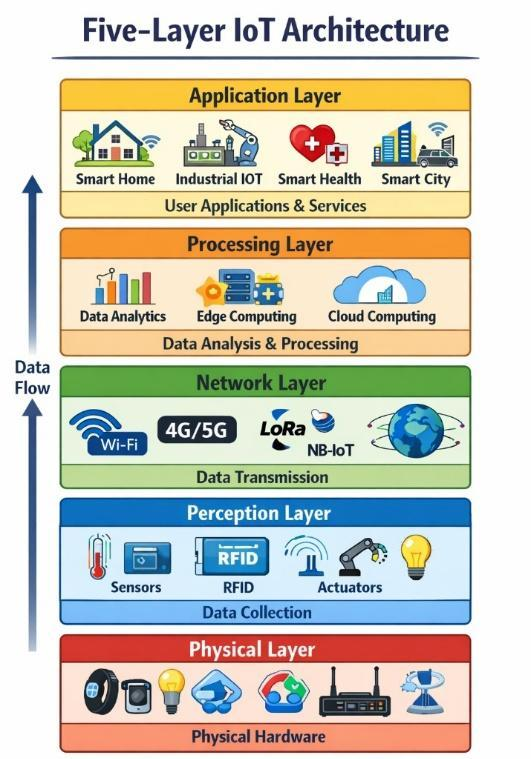
\includegraphics[width=0.50\columnwidth]{assets/images/faculty_pc_five_layer.jpg}
    \captionof{figure}{A layered view of IoT sensing, networking, processing, and applications.}
\end{minipage}
  \end{center}
\vspace{-0.9em}

  \subsection*{\centering\uppercase{Communication Models}}
  IoT devices exchange information through four common models:
  \begin{itemize}\justifying
    \item \textbf{Device-to-device:} nearby devices communicate directly through BLE, Zigbee, NFC, or another local link. This reduces latency and avoids dependence on a remote server.
    \item \textbf{Device-to-gateway:} a gateway aggregates data, translates protocols, enforces security, and forwards selected information to other networks or the cloud.
    \item \textbf{Device-to-cloud:} a device connects directly to an Internet service through Wi-Fi or cellular connectivity, simplifying central analytics and remote access.
    \item \textbf{Back-end data sharing:} authorised applications access common platform data through APIs, enabling cross-domain analytics and service integration.
  \end{itemize}

  \subsection*{\centering\uppercase{The IoT Protocol Stack}}
  IoT communication follows a layered stack adapted to devices with limited memory, power, and packet size. The physical layer defines modulation, spectrum, and signal transmission. The data-link layer controls framing, channel access, link addressing, and error detection. Technologies include Ethernet, Wi-Fi, BLE, IEEE 802.15.4, and LoRa.

  \noindent
  At the network layer, IPv6 provides addressing, 6LoWPAN compresses and fragments IPv6 packets for constrained links, and the Routing Protocol for Low-Power and Lossy Networks (RPL) supports multi-hop routing [1--3]. TCP offers reliable connection-oriented transport, whereas UDP reduces overhead and is often paired with lightweight application protocols. TLS protects TCP sessions, while DTLS provides comparable protection for datagram communication.

  \begin{center}
\vspace{-0.9em}
\begin{minipage}{0.98\columnwidth}
\centering
    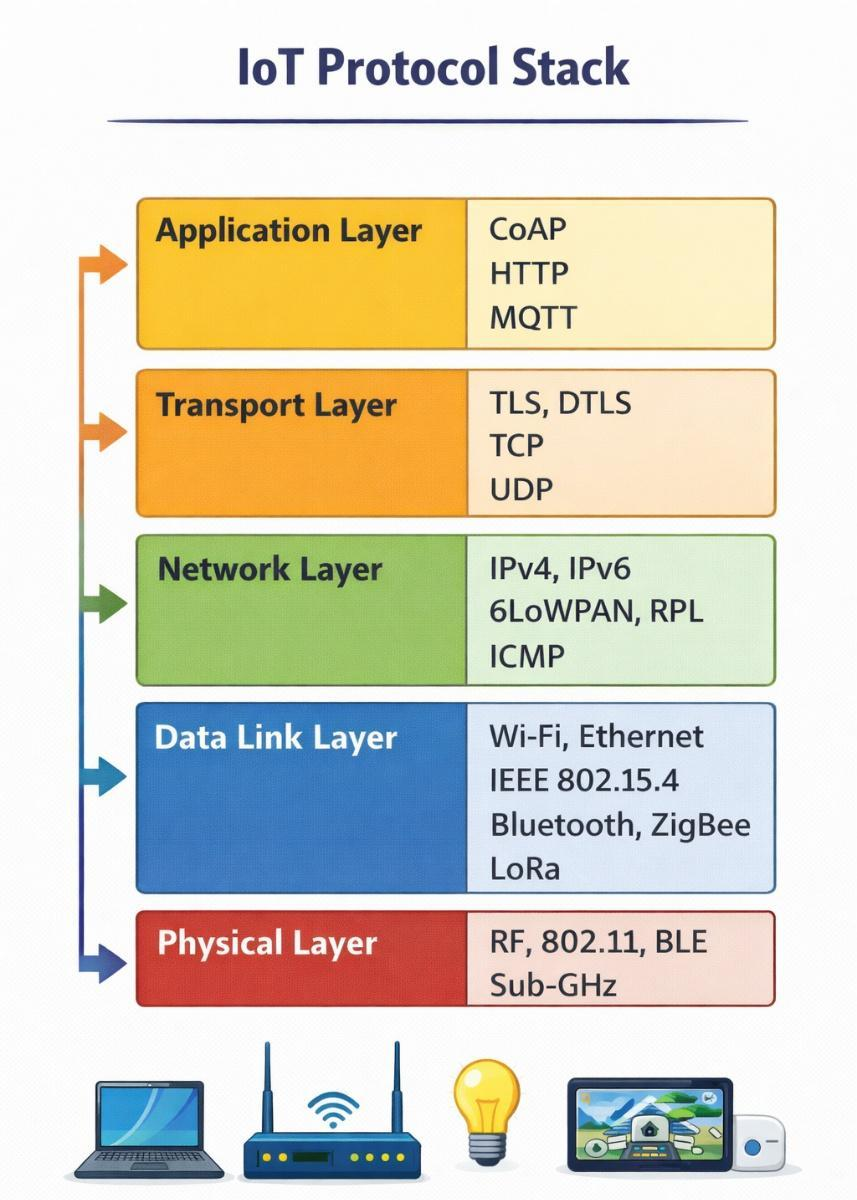
\includegraphics[width=0.70\columnwidth]{assets/images/faculty_pc_protocol_stack.jpg}
    \captionof{figure}{Protocols and technologies across a representative IoT stack.}
\end{minipage}
  \end{center}
\vspace{-0.9em}

  \needspace{4\baselineskip}
  \subsection*{\centering\uppercase{Short-Range Connectivity}}
  BLE operates in the 2.4-GHz band and is designed for small data exchanges with long battery life. It is widely used in wearables, beacons, fitness devices, and health monitors. Zigbee builds low-data-rate mesh networks over IEEE 802.15.4, allowing messages to pass through intermediate nodes. Z-Wave uses sub-GHz spectrum in home-automation networks, reducing interference from crowded 2.4-GHz systems.

  \noindent
  The choice among these technologies depends on topology, payload size, battery target, commissioning method, interoperability, security, and the availability of a gateway. A mesh extends coverage but increases routing and maintenance complexity.

  \subsection*{\centering\uppercase{Wide-Area Connectivity}}
  Wi-Fi offers relatively high throughput within homes, campuses, and industrial sites but normally consumes more power than constrained-radio solutions. Cellular systems provide managed infrastructure, mobility, and broad coverage. NB-IoT targets low-throughput devices requiring deep coverage and long battery life, while LTE-M supports higher rates and mobility.

  \noindent
  Low-Power Wide-Area Network (LPWAN) technologies such as LoRaWAN connect distant sensors that send small payloads infrequently. They are effective for soil monitoring, utility metering, and logistics, but are not designed for video or continuous low-latency control. Engineers must account for duty-cycle limits, link budget, gateway density, spectrum rules, and downlink capacity.

\end{multicols}

\begin{table}[!b]
\noindent\hfill\begin{minipage}{0.48\textwidth}
\raggedright
Table~1 summarizes representative IoT communication technologies and their design trade-offs.\par
\end{minipage}\par
\centering
\caption{Representative IoT communication technologies and design trade-offs.}
\normalsize
  \setlength{\tabcolsep}{2.5pt}
  \renewcommand{\arraystretch}{1.8}
  \begin{tabular}{@{}>{\bfseries\RaggedRight\arraybackslash}p{0.16\textwidth}
                      >{\Centering\arraybackslash}p{0.14\textwidth}
                      >{\Centering\arraybackslash}p{0.12\textwidth}
                      >{\RaggedRight\arraybackslash}p{0.20\textwidth}
                      >{\RaggedRight\arraybackslash}p{0.25\textwidth}@{}}
    \toprule
    \textbf{Technology} & \textbf{Typical Range} & \textbf{Energy Use} & \textbf{Strength} & \textbf{Representative Use} \\
    \midrule
    BLE & Short & Very low & Phone compatibility and low-power operation & Wearables and medical sensors \\
    Zigbee / IEEE 802.15.4 & Short to multi-hop & Low & Mesh networking and many local nodes & Smart lighting and building control \\
    Wi-Fi & Local-area & Moderate to high & High throughput and direct IP connectivity & Cameras, appliances, and gateways \\
    LoRaWAN & Long & Very low & Long range with small, infrequent payloads & Agriculture and environmental sensing \\
    NB-IoT / LTE-M & Wide-area & Low to moderate & Managed cellular coverage and mobility & Metering, logistics, and asset tracking \\
    5G & Wide-area & Varies & High capacity, mobility, and low-latency services & Vehicles, automation, and massive IoT \\
    \bottomrule
  \end{tabular}
\end{table}
\newpage

\noindent\begin{minipage}{\textwidth}
\centering
\captionof{table}{Comparison of common IoT application protocols.}
\scriptsize
  \setlength{\tabcolsep}{2.5pt}
  \renewcommand{\arraystretch}{1.12}
  \begin{tabular}{@{}>{\bfseries\RaggedRight\arraybackslash}p{0.16\textwidth}
                      >{\RaggedRight\arraybackslash}p{0.18\textwidth}
                      >{\Centering\arraybackslash}p{0.11\textwidth}
                      >{\RaggedRight\arraybackslash}p{0.20\textwidth}
                      >{\RaggedRight\arraybackslash}p{0.22\textwidth}@{}}
    \toprule
    \textbf{Protocol} & \textbf{Communication Pattern} & \textbf{Transport} & \textbf{Main Advantage} & \textbf{Typical Placement} \\
    \midrule
    MQTT & Publish--subscribe through a broker & TCP & Lightweight telemetry with selectable delivery QoS & Sensors, gateways, and cloud brokers \\
    CoAP & REST request--response and observation & UDP & Compact headers and constrained-device support & Local constrained IP networks \\
    HTTP/HTTPS & REST request--response & TCP & Universal web and cloud compatibility & Gateways, dashboards, and cloud APIs \\
    AMQP & Queues, routing, and publish--subscribe & TCP & Reliable enterprise messaging & Back-end and industrial integration \\
    \bottomrule
  \end{tabular}
\end{minipage}
\par\vspace{4pt}
\noindent\begin{minipage}{0.48\textwidth}
\raggedright
Table~2 compares common IoT application protocols and their typical placements.\par
\end{minipage}
\par\vspace{4pt}

\begin{multicols}{2}

  \subsection*{\centering\uppercase{Application-Layer Protocols}}
  \subsubsection*{MQTT}
  MQTT uses a publish--subscribe model. Devices publish messages to named topics through a broker, and subscribers receive topics of interest. This decouples producers and consumers and supports scalable telemetry. MQTT defines QoS 0 (at most once), QoS 1 (at least once), and QoS 2 (exactly once), trading overhead for delivery assurance [4].

  \subsubsection*{CoAP}
  The Constrained Application Protocol (CoAP) follows a REST-style request--response model similar to HTTP but normally uses UDP. Compact binary headers, multicast support, resource observation, and DTLS or object security make it suitable for constrained nodes [5].

  \subsubsection*{HTTP and AMQP}
  HTTP/HTTPS remains common between gateways, web applications, and cloud platforms because tools and services support it universally. Its overhead may be excessive for very constrained endpoints. AMQP provides reliable message queuing and routing for enterprise and industrial integration where richer broker functionality is required.

  \subsection*{\centering\uppercase{Quality of Service}}
  IoT performance is measured through latency, jitter, throughput, packet loss, reliability, and availability. Requirements vary sharply: a soil sensor may tolerate minutes of delay, while a protection relay or robotic controller may require deterministic response. QoS must therefore be designed across the radio, scheduling, routing, transport, application, and computing layers.

  \subsection*{\centering\uppercase{Security Across the Stack}}
  {\justifying
    IoT devices often operate unattended, handle sensitive data, and control physical equipment. Major threats include spoofing, replay, malware, tampering, denial-of-service, and insecure firmware; one compromised endpoint can expose a wider network.

    \noindent
    Defence requires unique identities, secure boot and key storage, signed updates, least privilege, and removal of default passwords. AES, ECC, TLS or DTLS, segmentation, monitoring, certificate management, vulnerability disclosure, and long-term update support provide layered protection [6].\par
  }

  \subsection*{\centering\uppercase{Interoperability and Standardisation}}
  Heterogeneous devices must agree on radio interfaces, addressing, message formats, discovery, security, and application semantics. IEEE develops important physical and MAC standards; the IETF specifies Internet protocols; 3GPP standardises cellular systems; the ITU coordinates international telecommunications; and industry alliances define application profiles.

  \noindent
  Protocol compliance alone does not guarantee interoperability. Two devices may use MQTT but publish incompatible topic structures or data units. Common information models, schemas, APIs, testing programmes, and device-management conventions are needed to achieve plug-and-play behaviour.

  \subsection*{\centering\uppercase{Cloud, Edge, and Fog Communication}}
  Cloud platforms provide scalable storage, analytics, visualisation, fleet management, and integration with business systems. Sending every sample to a distant cloud, however, can increase latency, bandwidth cost, and privacy exposure.

  \noindent
  Edge computing places processing near sensors. A gateway can filter noise, aggregate samples, detect anomalies, and execute urgent control even when the Internet connection is unavailable. Fog architectures distribute these functions across several intermediate nodes. Practical designs divide work according to urgency, computation, energy, privacy, and the value of retaining raw data.

  \begin{center}
\vspace{-0.9em}
\begin{minipage}{0.98\columnwidth}
\centering
    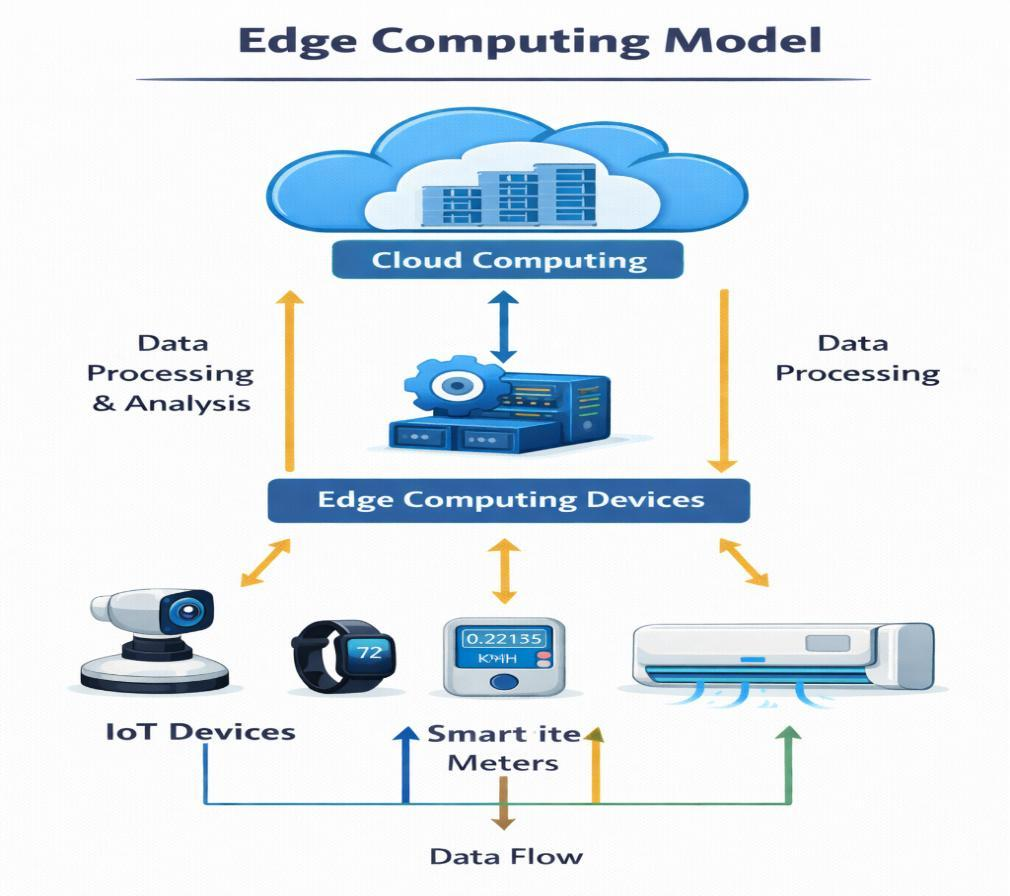
\includegraphics[width=0.75\columnwidth]{assets/images/faculty_pc_edge.jpg}
    \captionof{figure}{Edge nodes process time-sensitive data near IoT devices while coordinating with cloud services.}
\end{minipage}
  \end{center}
\vspace{-0.9em}

  \subsection*{\centering\uppercase{Industrial IoT}}
  Industrial IoT connects machines, robots, instruments, controllers, and supervisory platforms. Representative technologies include Modbus, OPC UA, PROFINET, and EtherCAT. Unlike consumer telemetry, industrial communication may demand bounded latency, deterministic scheduling, high availability, functional safety, and operation alongside legacy equipment.

  \noindent
  Predictive maintenance illustrates the value of IIoT: vibration and temperature sensors feed edge analytics that identify abnormal behaviour before a machine fails. The network must preserve time synchronisation, data integrity, and service continuity without allowing remote connectivity to weaken plant security.

  \subsection*{\centering\uppercase{Applications}}
  In smart agriculture, soil and climate sensors communicate through LPWAN to control irrigation and improve resource use. Smart-city systems coordinate traffic signals, parking, lighting, and waste collection. Healthcare devices monitor heart rate, blood pressure, oxygen saturation, and movement, requiring dependable delivery, privacy, and clinical oversight. Similar networking principles support asset tracking, environmental observation, connected vehicles, and intelligent buildings.

  \subsection*{\centering\uppercase{Emerging Paradigms}}
  \begin{itemize}\justifying
    \item \textbf{6G and massive machine communication:} future systems aim to integrate terrestrial, aerial, and satellite networks with extremely dense sensing and context-aware services.
    \item \textbf{AI-assisted networking:} learning systems can predict faults, estimate congestion, optimise routing, allocate spectrum, and detect abnormal traffic.
    \item \textbf{Blockchain and distributed trust:} tamper-evident ledgers may support shared audit trails and decentralised identity, although computation and storage overhead must be justified.
    \item \textbf{Satellite IoT:} low-Earth-orbit connectivity can reach farms, oceans, pipelines, and remote infrastructure outside terrestrial coverage.
    \item \textbf{Energy-aware networking:} wake-up radios, adaptive duty cycles, energy harvesting, and lightweight protocols extend unattended device life.
  \end{itemize}

  \subsection*{\centering\uppercase{Design Challenges}}
  Large deployments face address management, radio coexistence, changing topology, battery replacement, data overload, vendor fragmentation, physical exposure, and long device lifetimes. Scalable management must automate onboarding, configuration, monitoring, credential rotation, firmware updates, and secure retirement. The technically strongest protocol is not necessarily the best choice if it cannot meet cost, energy, coverage, maintenance, or interoperability constraints.

  \subsection*{\centering\uppercase{Conclusion}}
  IoT networking combines embedded design, radio communication, Internet protocols, distributed computing, security, and application engineering. Layered architectures and gateways help integrate heterogeneous devices, while technologies such as BLE, Zigbee, Wi-Fi, LPWAN, cellular IoT, MQTT, CoAP, IPv6, and RPL address different operating conditions.

  \noindent
  Future systems will increasingly combine edge intelligence, cloud-scale coordination, AI-assisted management, advanced cellular networks, and satellite coverage. Reliable IoT design therefore requires deliberate trade-offs among range, rate, latency, energy, reliability, scalability, interoperability, security, and lifecycle support. Communication is not merely a connection between devices; it is the foundation that allows sensing, computation, and action to operate as one intelligent system.

  \subsection*{\centering\uppercase{References}}
  {\small
  \begin{justify}
    \begin{enumerate}[label={\relax[\arabic*]},leftmargin=*,labelsep=0.5em,itemsep=0.20em,parsep=0pt]
      \item J. Hui and P. Thubert, \textit{Compression Format for IPv6 Datagrams over IEEE 802.15.4-Based Networks}, IETF RFC 6282, 2011.
      \item IEEE, \textit{IEEE Standard for Low-Rate Wireless Networks}, IEEE 802.15.4.
      \item T. Winter et al., \textit{RPL: IPv6 Routing Protocol for Low-Power and Lossy Networks}, IETF RFC 6550, 2012.
      \item OASIS, \textit{MQTT Version 5.0}, OASIS Standard, 2019.
      \item Z. Shelby, K. Hartke, and C. Bormann, \textit{The Constrained Application Protocol (CoAP)}, IETF RFC 7252, 2014.
      \item M. Fagan et al., \textit{IoT Device Cybersecurity Capability Core Baseline}, NISTIR 8259A, 2020.
      \item 3GPP, \textit{Cellular System Support for Ultra-Low Complexity and Low Throughput Internet of Things}.
      \item OPC Foundation, \textit{OPC Unified Architecture Specification}.
    \end{enumerate}
  \end{justify}}
\end{multicols}
\endgroup
